\subsection{Open Vivado 2023}
    
    \ifpdf
        \begin{figure}[H]
        Open Vivado and click on Create Project under the quick start menu. 

            \centering
            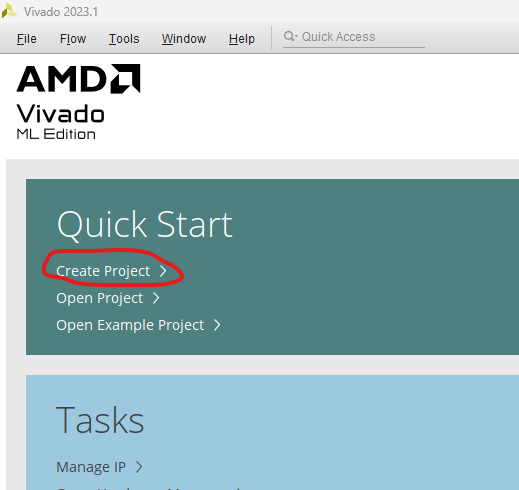
\includegraphics[width=5cm]{Images/Vivado_CreateProject.png}
            \caption{Select Create Project}
            \label{fig:enter-label}
        \end{figure}
    \else
        \HCode{<video width="320" height="240" controls>
          <source src="Images/CreateProject_Vivado2023.mp4" type="video/mp4">
          <img src="Images/Vivado_CreateProject.png" alt="Video Shows the button press for the create project">
          Your browser does not support the video tag.
        </video>}
    \fi

\subsection{Create a New Project}
    Follow along with the Create a New Project Wizard.\\
    \vspace{1cm}
    
\includegraphics[width = 1cm]{Images/Alert Icon.png} \textbf{
    If you are working on the lab computers, ensure your project is saved on your Desktop!
    This is due to file latency with the H drive preventing tools from behaving correctly.
    You will need to also ensure you backup your project as the drive gets cleaned intermittently.
    DO NOT SAVE TO THE TEMP DRIVE as that is shared between users.}

    \vspace{1cm}
    
\ifpdf
    \begin{figure}[H]
        \centering
        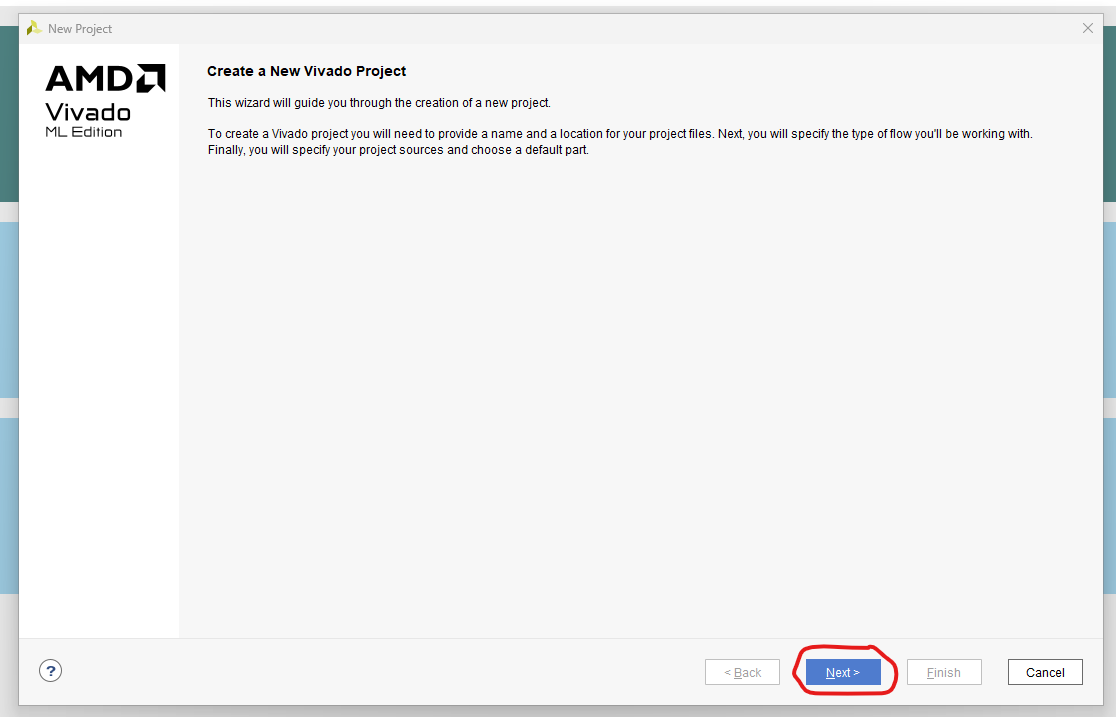
\includegraphics[width=9cm]{Images/CreateProjectImages/Vivado_CreateProject_Page1.png}
        \caption{Follow through with create project wizard.}
        \label{fig:enter-label}
    \end{figure}
    \begin{figure}[H]
        \centering
        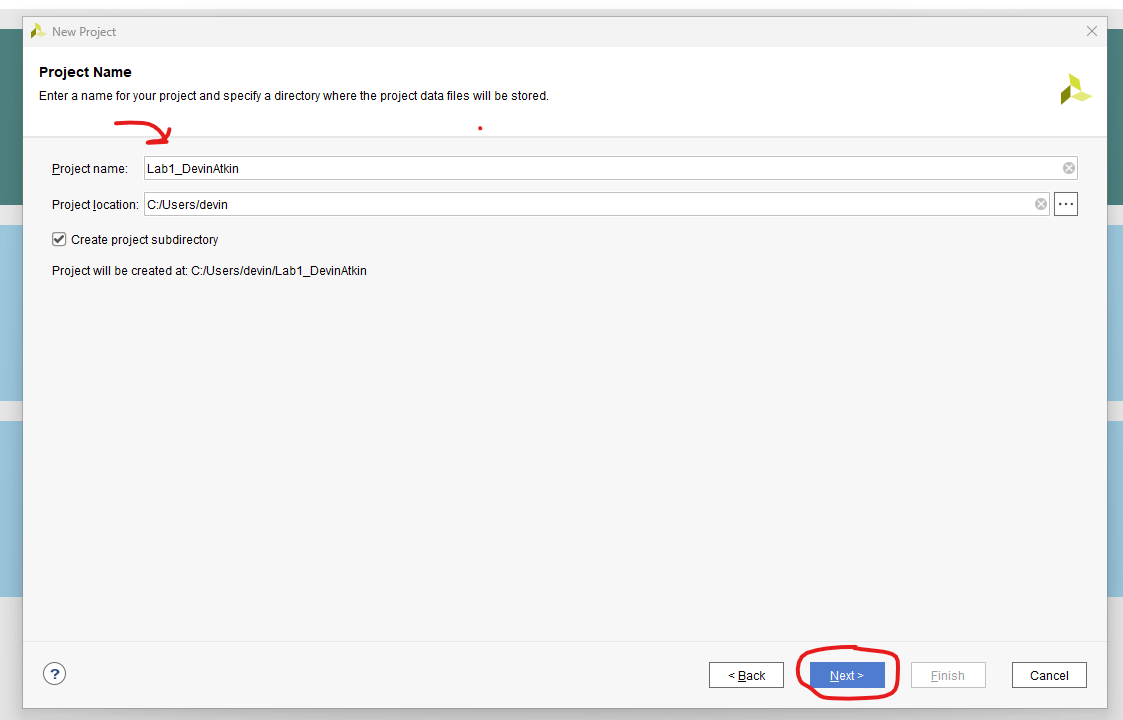
\includegraphics[width=9cm]{Images/CreateProjectImages/Vivado_CreateProject_Page2.png}
        \caption{Give  your project a name.}
        \label{fig:enter-label}
        \raggedright
        \vspace{0.5cm}
        Use the structure 
        \textbf{LabX\_FirstName\_LastName}
        for your project name. The marking will rely on the lab names so variations may cause issues with incorrect marking! 
    \end{figure}


    \begin{figure}[H]
        \centering
        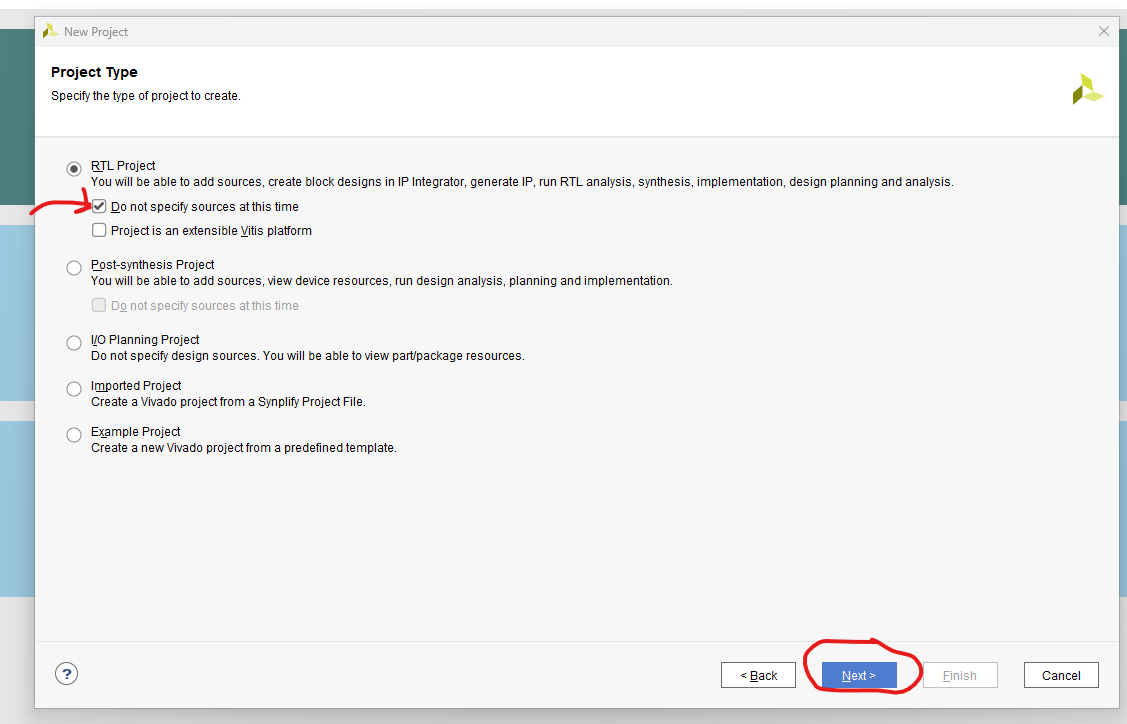
\includegraphics[width=9cm]{Images/CreateProjectImages/Vivado_CreateProject_Page3.png}
        \caption{Select RTL Project}
        \label{fig:enter-label}
        \raggedright
        Select RTL Project, and check the option to not include sources at this time. You will import the lab code once the project is fully setup.

    \end{figure}

    \begin{figure}[H]
        \centering
        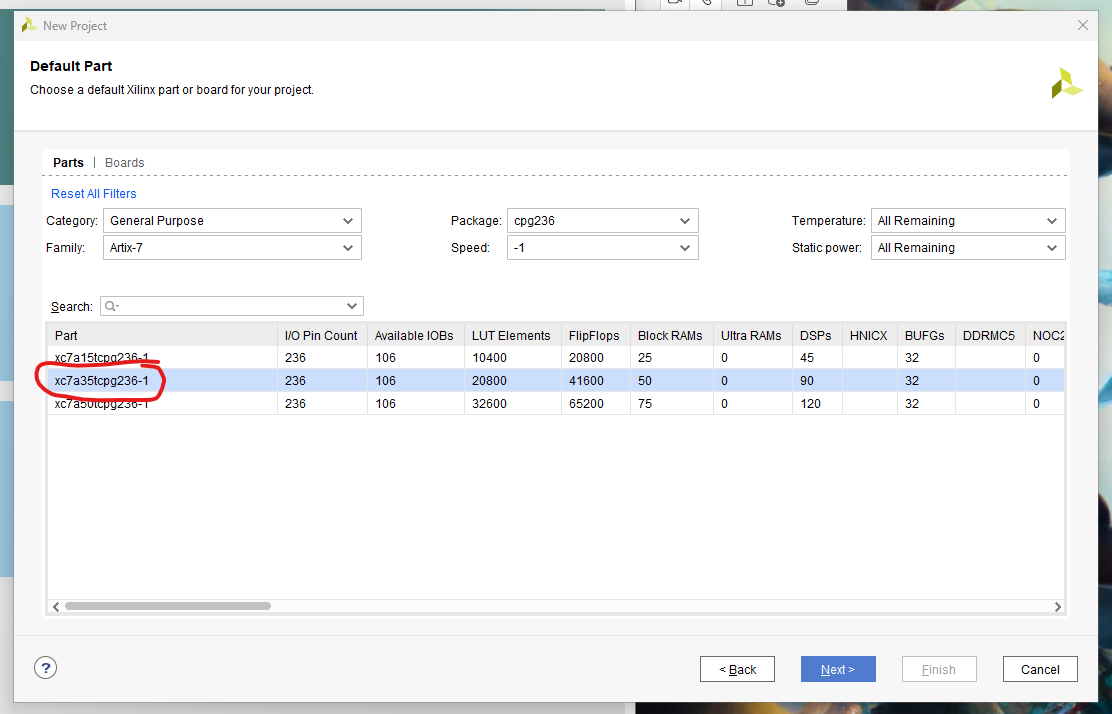
\includegraphics[width=9cm]{Images/CreateProjectImages/Vivado_CreateProject_Page4.png}
        \caption{Select the FPGA used by the Basys3}
        \label{fig:enter-label}
        \raggedright
        \vspace{0.5cm}
        The Correct FPGA is xc7a35tcpg236-1. Select the following to narrow the options.
        \begin{itemize}
            \item Category: General Purpose
            \item Family: Artix-7
            \item Package: cpg236
            \item Speed: -1
            \item Of the last 3 items in the list the center one should be correct.
        \end{itemize}
    \end{figure}
    The Basys 3 board uses an Artix-7 FPGA, selecting from the available list it is the xc7a35tcpg236-1. You can either use the search functionality or narrow the selection by choosing the appropriate category, family, package, and speed. Note that there are 3 FPGAs available with this selection, they represent different sizes of the same chip, in a design environment you would want to optimize to fit onto the smallest possible chip to minimize costs. FPGAs are expensive components; however, comparing the price of different models, the cost for the Artix-7 chips varies from ~\$50 to ~\$800. This is strong motivation to optimize your design. 

    \begin{figure}[H]
        \centering
        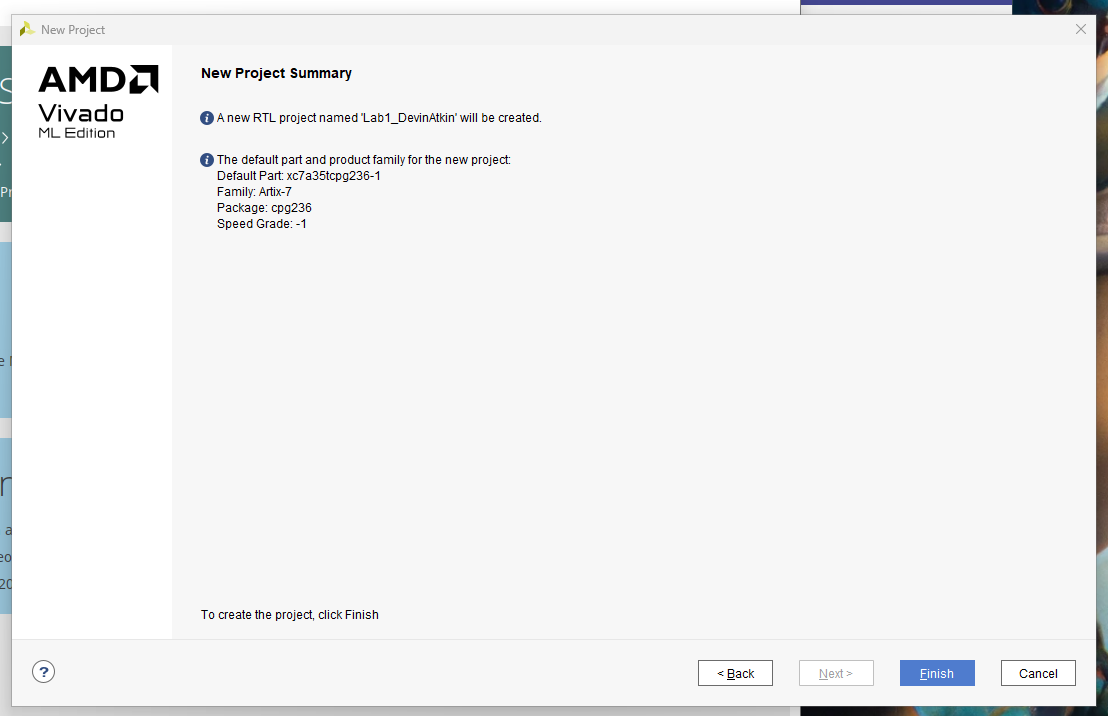
\includegraphics[width=9cm]{Images/CreateProjectImages/Vivado_CreateProject_Page5.png}
        \caption{Finish the project creation}
        \label{fig:enter-label}
    \end{figure}
    With this you should have everything setup and you can begin the lab. Verify the details listed for the project on this page and press finish to create the project. 
\else
    \HCode{<video width="320" height="240" controls>
    <source src="Images/CreateProject_Vivado2023.mp4" type="video/mp4">
    <img src="Images/Vivado_CreateProject.png" alt="Video Shows the button press for the create project">
    Your browser does not support the video tag. (Still need to update this to a new video)
    </video>}
\fi

\subsection{Adding Lab Files}
You now have a project created. You are going to need to add a handful of files to simulate and execute the project provided for this lab. The following files are provided with this lab \textit{Basys3\_Lab1\_Constraints.xdc, top\_level.sv, crc\_calc.sv, crc\_statemachine.sv, tb\_crc\_statemachine.sv, tb\_crc\_calc.sv, and tb\_top\_level.sv}. To add them to the project click on the plus sign in the sources window.

\ifpdf
    \begin{figure}[H]
        \centering
        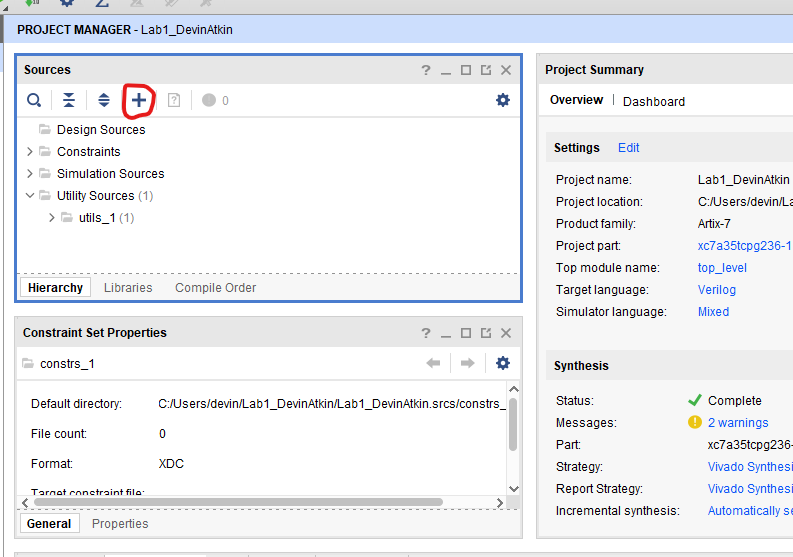
\includegraphics[width=9cm]{Images/CreateBitstreamImages/Vivado_AddSources1.png}
        \caption{Press the plus icon to begin adding sources}
        \label{fig:enter-label}
        \raggedright
        \vspace{0.5cm}
        Press the plus icon to begin adding the provided files to the project. This will bring up the add file wizard which will allow you to add each file in turn or create new files.

    \end{figure}
    
    \begin{figure}[H]
        \centering
        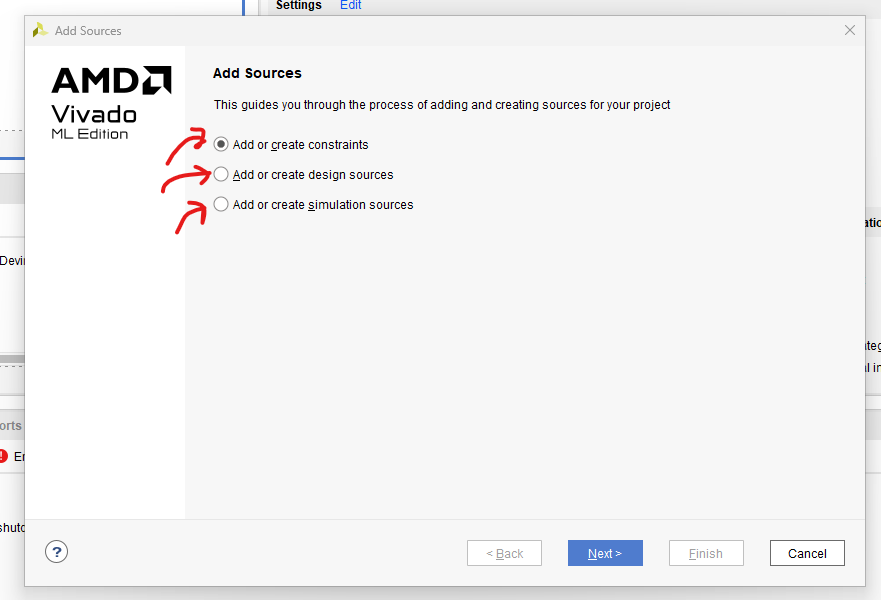
\includegraphics[width=9cm]{Images/CreateBitstreamImages/Vivado_AddSources_Page1.png}
        \caption{File Add Wizard}
        \label{fig:enter-label}
        \raggedright
        \vspace{0.5cm}
            When you press the button the Add sources tool will appear with three options.
    You'll need to repeat this step three times for the design sources (\textit{top\_level.sv, crc\_calc.sv, crc\_statemachine.sv}), simulation sources (\textit{tb\_top\_level.sv and tb\_crc\_calc.sv, tb\_crc\_statemachine.sv}), and constraints file (\textit{Basys3\_Lab1\_Constraints.xdc}). We'll explain what is in each of these files later.

    \end{figure}

    \begin{figure}[H]
        \centering
        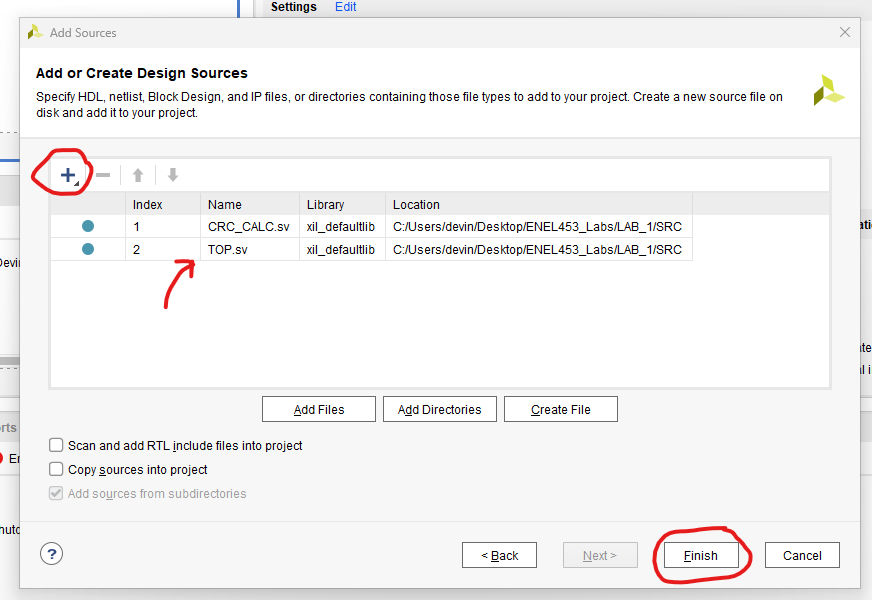
\includegraphics[width=9cm]{Images/CreateBitstreamImages/Vivado_AddSources_Page2.png}
        \caption{Select Add Files under the Plus}
        \label{fig:enter-label}
        \raggedright
        \vspace{0.5cm}
        Repeat this process for each option in turn. Hit next, select add files, and select the appropriate design sources, simulation sources, and constraints files respectively. After you have added all the provided files the design should be ready for generating a bitstream. \textbf{In the sources menu ensure that top\_level.sv is selected as the top, it will have 3 small squares next to it 
\includegraphics[height=4mm]{Images/CreateProjectImages/top_level_3Dots.png}. If it does not right click on the file in the sources menu and select Set as Top. This is the top of the design and will ensure that the bitstream is generated correctly. Vivado will often correctly select the top file when it is being added to the design. It is worth noting that top\_level or top is a fairly ubiquitous standard name for top cells in fpga projects.}
    \end{figure}

    
\else
    \HCode{<video width="320" height="240" controls>
    <source src="Images/CreateProject_Vivado2023.mp4" type="video/mp4">
    <img src="Images/Vivado_CreateProject.png" alt="Video Shows the button press for the create project">
    Your browser does not support the video tag. (Still need to update this to a new video)
    </video>}
\fi

\subsection{RTL View}
After adding your files you can check that the design is loaded correctly by opening up the RTL view. This represents your design
\begin{figure}[H]
    \centering
    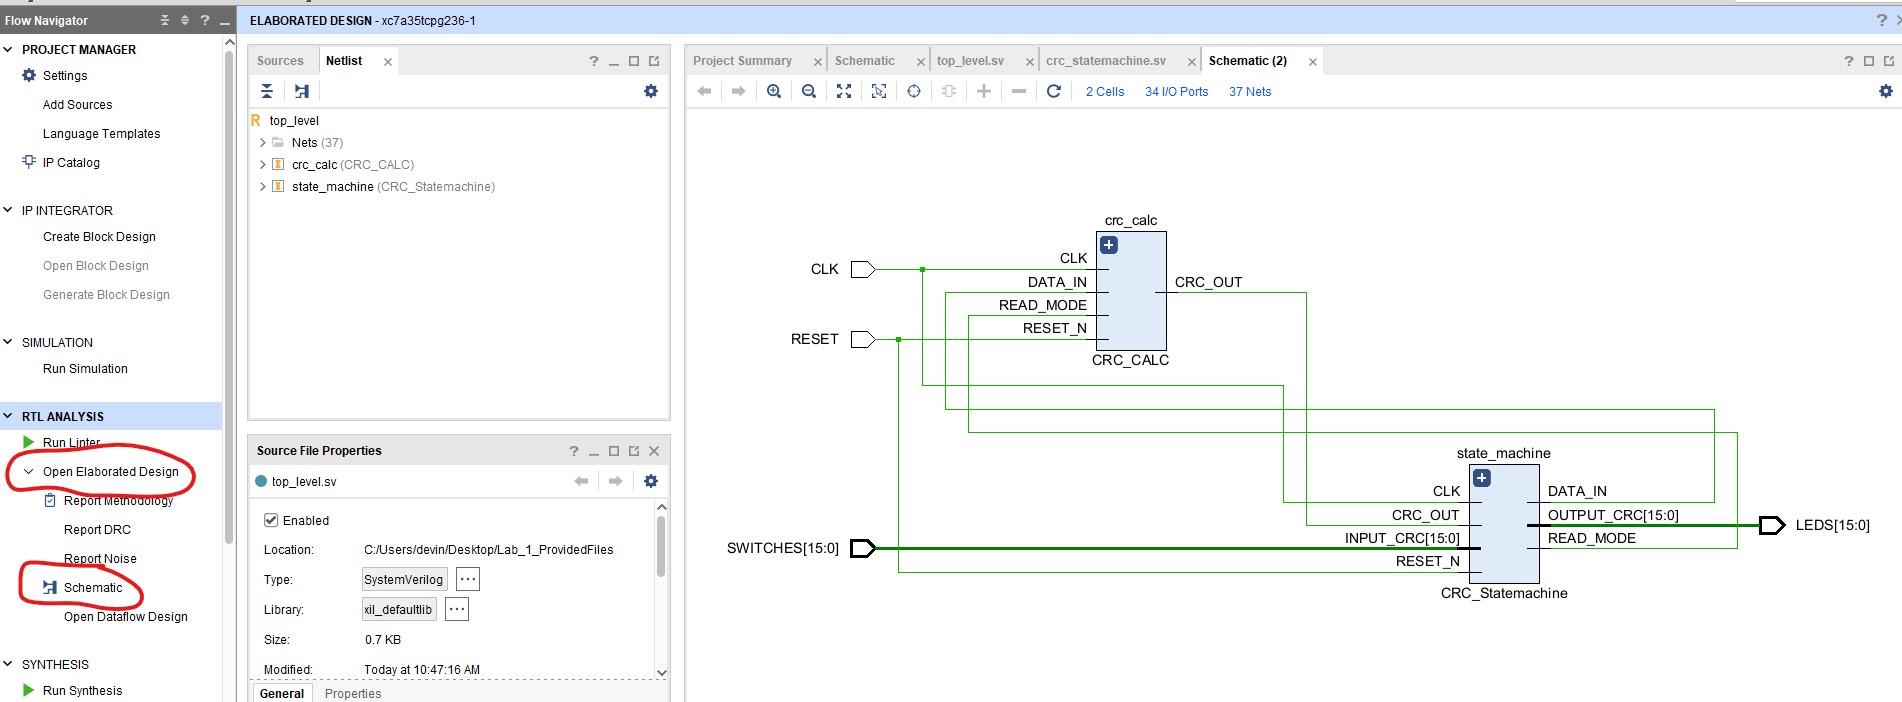
\includegraphics[width = 9cm] {Images/CreateBitstreamImages/OpenElaboratedDesign.jpg}
    \caption{Look at the RTL View}
    \label{fig:enter-label}
    \raggedright
    \vspace{0.5cm}
    Open the elaborated schematic by clicking open elaborated design, then clicking on schematic. This will compile the top level files and create a schematic representation of the design.
    You can click on the blocks in the design and it will expand out to show you the lower levels. Once finished with this lab \textbf{return to this view and include a screenshot in your design report.} Take note that no logic exists in this top level. While technically possible to have logic at any level, it is considered especially bad practice, the most logic that is considered acceptable is singular inverters. You'll need to add this to the design as part of the modifications in a later section. \\
    \vspace{0.5cm}
    
\includegraphics[height=1cm]{Images/Alert Icon.png}  \textbf{RTL view is one of the most useful tools for diagnosing problems in your FPGA design.} The RTL view represents the schematic view of your design, it is incredibly useful for confirming that you are creating the design as intended. When debugging larger designs it can be often worth restructuring larger elements to create blocks which have clear representations in the RTL view so that you can more easily diagnose issues. 
\end{figure}
\subsection{Synthesis and Implementation}
You'll remember that synthesis takes the HDL design and converts it into elements in the fpga, and then implementation takes those and maps it onto the actual fpga hardware.
\vspace{0.5cm}
\begin{figure}[H]
    \centering
    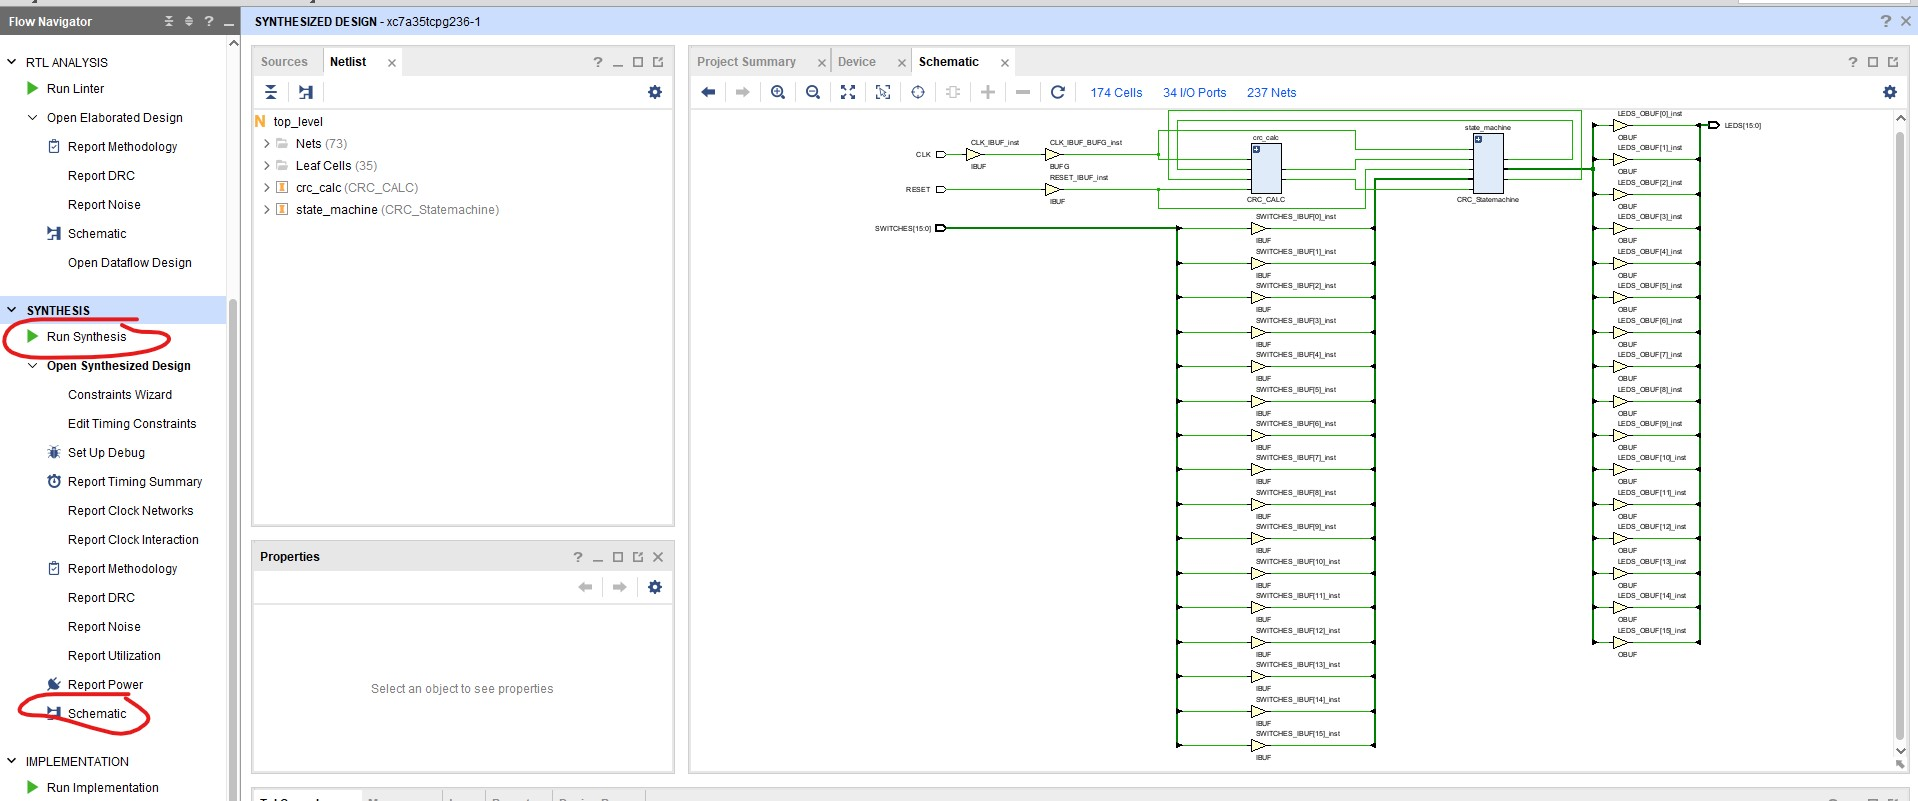
\includegraphics[width=9cm]{Images/CreateProjectImages/SynthesizeYourDesign.jpg}
    \caption{Run Synthesis}
    \label{fig:enter-label}
    \raggedright
    \vspace{0.5cm}
    Press Run Synthesis in the left hand panel. This will being up a dialog for starting synthesis, you go ahead and accept this immediately or change the number of jobs. It won't make a substantial difference in time now; however, on larger designs this will help speed up the process. Once you've run synthesis open the synthesized design and look at the schematic again, you'll notice that the logic gates have been replaced with LUTs.
\end{figure}

Once you're done looking at the elaborated design you'll want to run implementation. This will map the hardware onto the physical FPGA. This is where you'll need to grab your timing details.\\
\subsection{Implementation}
\begin{figure}[H]
    \centering
    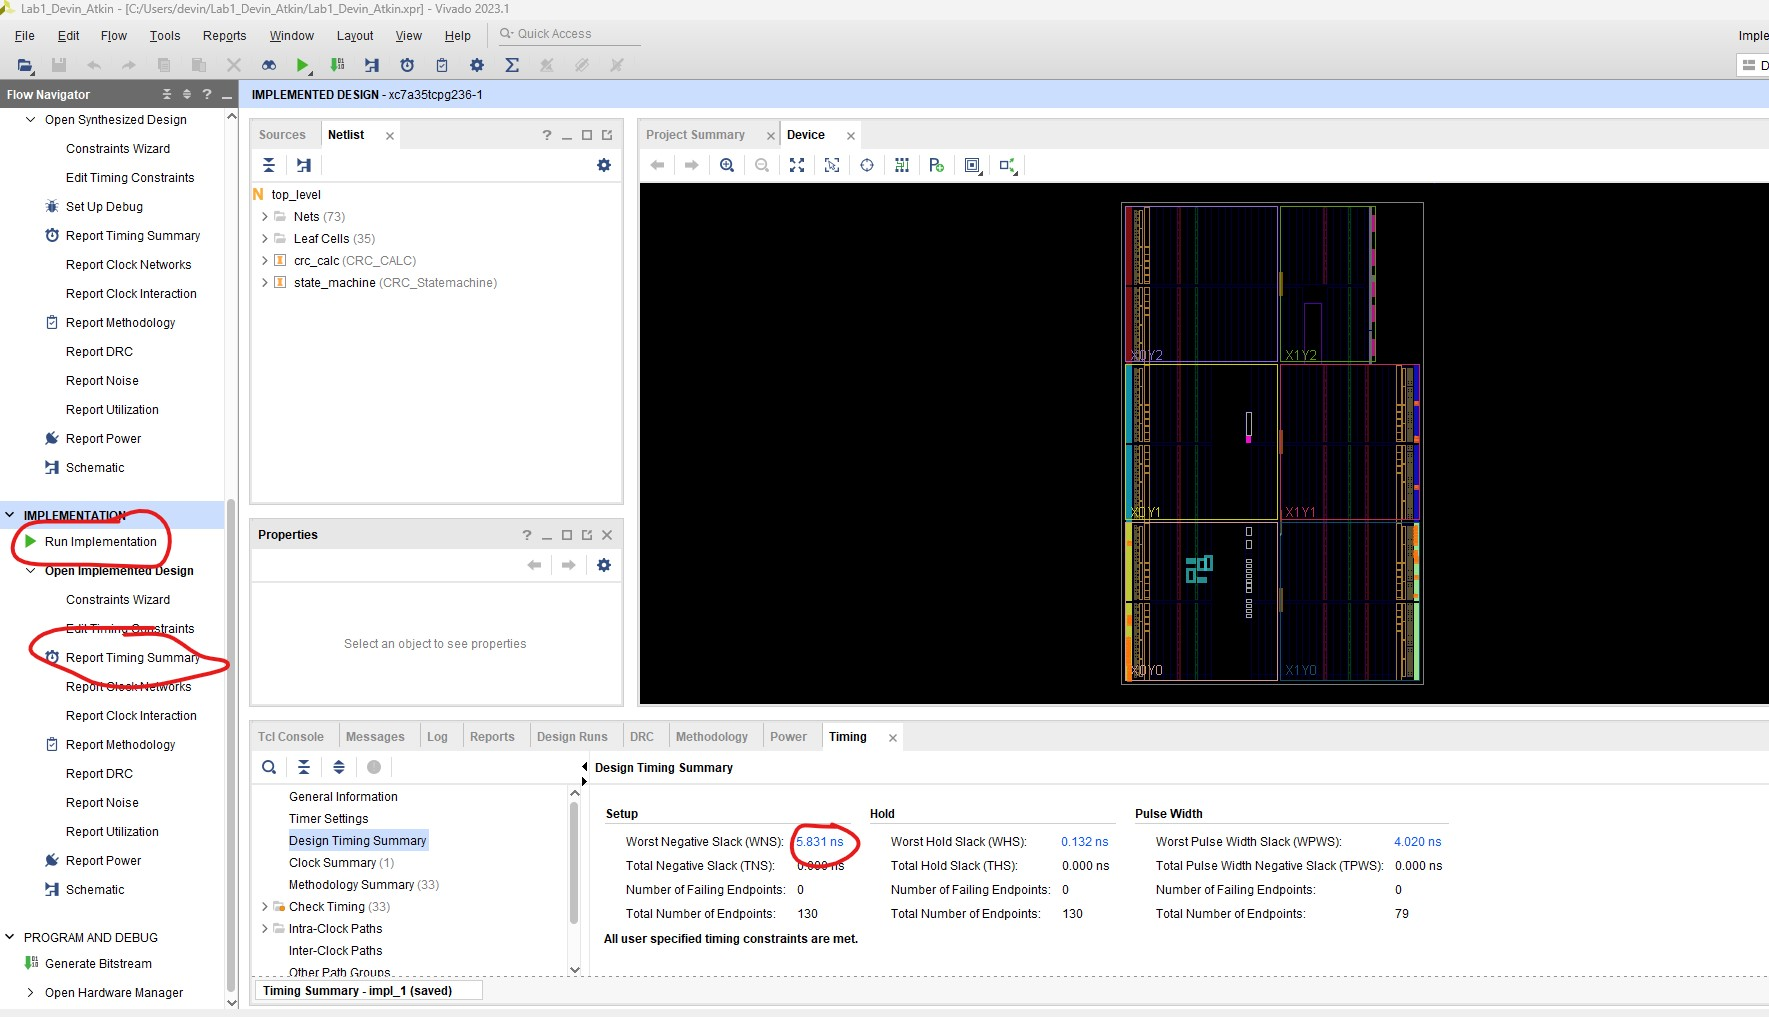
\includegraphics[width=9cm]{Images/CreateProjectImages/Implementation.jpg}
    \caption{Make sure to include your timing summary}
    \label{fig:enter-label}
\end{figure}
You will need to include the timing details on your lab design reports. You get this from the implementation. The timing summary should come up after implemention is run assuming you open the implemented design; however, if it doesn't you can get the timing summary by clicking \textit{Report Timing Summary} and then clicking ok for the default report. To Note, there is a separate timing report at the synthesis level which you don't necessarily need to pay attention to; however, if it fails to pass, implementation will almost definitely also fail to pass as well. 

\vspace{1cm}
\textbf{All of your designs must pass timing}. This means that they must be able to run at at least the 100MHz built in clock used by the Basys3. You are unlikely to run into timing issues on labs 1 and 2; however, this may become a challenge on labs 3 and 4 if you aren't careful when it comes to doing math. 

\vspace{0.5cm}
Use the following equation to calculate the maximum operating frequency for your design.
\[f_{max} = \frac{1}{t_{per}-t_{wns}} \]
Where \(f_{max}\) is the maximum operating frequency, \(t_{per}\) is the target period (in this case 10ns), and \(t_{wns}\) is the worst negative slack for the given implementation. The target period is determined by the clock speed of the design, this is defined in the constraints file for the project. You can see the clock being created here:

\begin{small}
\begin{verbatim}
## Clock signal
set_property PACKAGE_PIN W5 [get_ports CLK]							
set_property IOSTANDARD LVCMOS33 [get_ports CLK]
create_clock -add -name sys_clk_pin -period 10.00 -waveform {0 5} [get_ports CLK]
\end{verbatim}
\end{small}
The period is after the -period and is expressed in nanoseconds. However, this is determined by the crystal oscillator on the Basys3. If we were performing logic which required a slower clock speed, we would have to use either clock dividers or a PLL on chip to generate the alternate frequency. 

